%%%%%%%%%%%%  Generated using docx2latex.com  %%%%%%%%%%%%%%

%%%%%%%%%%%%  v2.0.0-beta  %%%%%%%%%%%%%%

\documentclass[12pt]{article}
\usepackage{amsmath}
\usepackage{latexsym}
\usepackage{amsfonts}
\usepackage[normalem]{ulem}
\usepackage{soul}
\usepackage{array}
\usepackage{amssymb}
\usepackage{extarrows}
\usepackage{graphicx}
\usepackage[backend=biber,
style=numeric,
sorting=none,
isbn=false,
doi=false,
url=false,
]{biblatex}\addbibresource{bibliography.bib}

\usepackage{subfig}
\usepackage{wrapfig}
\usepackage{txfonts}
\usepackage{wasysym}
\usepackage{enumitem}
\usepackage{adjustbox}
\usepackage{ragged2e}
\usepackage[svgnames,table]{xcolor}
\usepackage{tikz}
\usepackage{longtable}
\usepackage{changepage}
\usepackage{setspace}
\usepackage{hhline}
\usepackage{multicol}
\usepackage{tabto}
\usepackage{float}
\usepackage{multirow}
\usepackage{makecell}
\usepackage{fancyhdr}
\usepackage[toc,page]{appendix}
\usepackage[hidelinks]{hyperref}
\usetikzlibrary{shapes.symbols,shapes.geometric,shadows,arrows.meta}
\tikzset{>={Latex[width=1.5mm,length=2mm]}}
\usepackage{flowchart}\usepackage[paperheight=11.0in,paperwidth=8.5in,left=1.19in,right=1.18in,top=1.04in,bottom=0.19in,headheight=1in]{geometry}
\usepackage[utf8]{inputenc}
\usepackage[T1]{fontenc}
\usepackage[spanish]{babel}
\TabPositions{0.5in,1.0in,1.5in,2.0in,2.5in,3.0in,3.5in,4.0in,4.5in,5.0in,5.5in,6.0in,}

\urlstyle{same}


 %%%%%%%%%%%%  Set Depths for Sections  %%%%%%%%%%%%%%

% 1) Section
% 1.1) SubSection
% 1.1.1) SubSubSection
% 1.1.1.1) Paragraph
% 1.1.1.1.1) Subparagraph


\setcounter{tocdepth}{5}
\setcounter{secnumdepth}{5}


 %%%%%%%%%%%%  Set Depths for Nested Lists created by \begin{enumerate}  %%%%%%%%%%%%%%


\setlistdepth{9}
\renewlist{enumerate}{enumerate}{9}
		\setlist[enumerate,1]{label=\arabic*)}
		\setlist[enumerate,2]{label=\alph*)}
		\setlist[enumerate,3]{label=(\roman*)}
		\setlist[enumerate,4]{label=(\arabic*)}
		\setlist[enumerate,5]{label=(\Alph*)}
		\setlist[enumerate,6]{label=(\Roman*)}
		\setlist[enumerate,7]{label=\arabic*}
		\setlist[enumerate,8]{label=\alph*}
		\setlist[enumerate,9]{label=\roman*}

\renewlist{itemize}{itemize}{9}
		\setlist[itemize]{label=$\cdot$}
		\setlist[itemize,1]{label=\textbullet}
		\setlist[itemize,2]{label=$\circ$}
		\setlist[itemize,3]{label=$\ast$}
		\setlist[itemize,4]{label=$\dagger$}
		\setlist[itemize,5]{label=$\triangleright$}
		\setlist[itemize,6]{label=$\bigstar$}
		\setlist[itemize,7]{label=$\blacklozenge$}
		\setlist[itemize,8]{label=$\prime$}



 %%%%%%%%%%%%  Header here  %%%%%%%%%%%%%%


\pagestyle{fancy}
\fancyhf{}
\chead{ {\fontsize{10pt}{12.0pt}\selectfont \uline{\ \ \ \ \ \ \ \ \ \ \  Comparativa de Gestores de Base de Datos No Relacionales $\bullet$ \textit{ julio 2020 $\bullet$  \tabto{1.65in}  \tabto{5.27in} }}\par}
\vspace{\baselineskip}
}
\renewcommand{\headrulewidth}{0pt}
\setlength{\topsep}{0pt}\setlength{\parindent}{0pt}
\renewcommand{\arraystretch}{1.3}


%%%%%%%%%%%%%%%%%%%% Document code starts here %%%%%%%%%%%%%%%%%%%%



\begin{document}
\begin{adjustwidth}{0.56in}{0.57in}
\section*{Comparativa de Gestores de Base de Datos No Relacionales}
\addcontentsline{toc}{section}{Comparativa de Gestores de Base de Datos No Relacionales}
\end{adjustwidth}

\begin{adjustwidth}{0.56in}{0.57in}
\section*{Belizario Mamani, Loja Mamani, Lizárraga Paolo, Kenyi Chino}
\addcontentsline{toc}{section}{Belizario Mamani, Loja Mamani, Lizárraga Paolo, Kenyi Chino}
\end{adjustwidth}

\begin{adjustwidth}{0.56in}{0.57in}
\section*{July 08, 2020}
\addcontentsline{toc}{section}{July 08, 2020}
\end{adjustwidth}

\begin{adjustwidth}{0.56in}{0.57in}
\subsection*{Abstract}
\addcontentsline{toc}{subsection}{Abstract}
\end{adjustwidth}


\vspace{\baselineskip}
{\fontsize{10pt}{12.0pt}\selectfont There are two types of databases, relational and non-relational. In this article, we will see the comparison between two non-relational database managers (NoSQL), their differences, advantages, disadvantages and characteristics of each of the two managers.\par}\par


\vspace{\baselineskip}

\vspace{\baselineskip}

\vspace{\baselineskip}
\begin{multicols}{2}
\section{Introduccion}
\begin{justify}
{\fontsize{9pt}{10.8pt}\selectfont En este artículo veremos los cuadrantes del Agile Testing, que está formado por 4, el lado izquierdo es sobre guiar el desarrollo y realizar pruebas en forma temprana, el lado derecho es sobre la evaluación del producto y aprender lo que aún falta.\par}
\end{justify}\par


\vspace{\baselineskip}

\vspace{\baselineskip}
\section{RESUMEN}
\begin{justify}
{\fontsize{9pt}{10.8pt}\selectfont Existen dos tipos de bases de datos, las relacionales y no relacionales. En este artículo veremos la comparativa entre dos gestores de bases de datos NO relacionales (NoSQL), sus diferencias, ventajas, desventajas y características de cada uno de los dos gestores.\par}
\end{justify}\par


\vspace{\baselineskip}
\section{TITULO}

\vspace{\baselineskip}{\fontsize{9pt}{10.8pt}\selectfont \ \ \ \ \ \ \ \ \ \ \ \ \ \ \  Cuadrantes de pruebas agiles.\par}\par


\vspace{\baselineskip}
\section{AUTORES}

\vspace{\baselineskip}
{\fontsize{9pt}{10.8pt}\selectfont Los autores de este trabajo final de unidad son:\par}\par


\vspace{\baselineskip}


%%%%%%%%%%%%%%%%%%%% Figure/Image No: 1 starts here %%%%%%%%%%%%%%%%%%%%

\begin{figure}[H]		
\includegraphics[width=1.75in,height=1.44in]{./media/image1.png}
\end{figure}


%%%%%%%%%%%%%%%%%%%% Figure/Image No: 1 Ends here %%%%%%%%%%%%%%%%%%%%

\begin{itemize}
	\item {\fontsize{9pt}{10.8pt}\selectfont Paolo Lizárraga\par}\par


\end{itemize}
\vspace{\baselineskip}

%%%%%%%%%%%%%%%%%%%% Figure/Image No: 2 starts here %%%%%%%%%%%%%%%%%%%%

\begin{figure}[H]		
\includegraphics[width=1.84in,height=1.72in]{./media/image2.png}
\end{figure}


%%%%%%%%%%%%%%%%%%%% Figure/Image No: 2 Ends here %%%%%%%%%%%%%%%%%%%%

\begin{itemize}
	\item {\fontsize{9pt}{10.8pt}\selectfont Anthony Belizario\par}\par


\vspace{\baselineskip}

\vspace{\baselineskip}

\vspace{\baselineskip}
	\item {\fontsize{9pt}{10.8pt}\selectfont Daniel Loja\par}\par



%%%%%%%%%%%%%%%%%%%% Figure/Image No: 3 starts here %%%%%%%%%%%%%%%%%%%%

\begin{figure}[H]		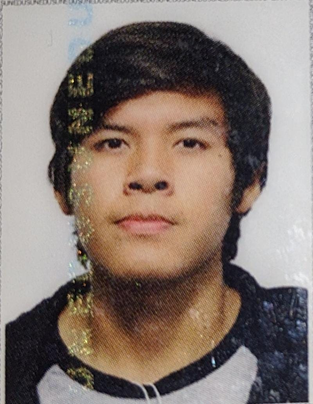
\includegraphics[width=2.01in,height=1.86in]{./media/image3.png}
\end{figure}


%%%%%%%%%%%%%%%%%%%% Figure/Image No: 3 Ends here %%%%%%%%%%%%%%%%%%%%

\par

	\item {\fontsize{9pt}{10.8pt}\selectfont Kenyi chino\par}
\end{itemize}\par



%%%%%%%%%%%%%%%%%%%% Figure/Image No: 4 starts here %%%%%%%%%%%%%%%%%%%%

\begin{figure}[H]		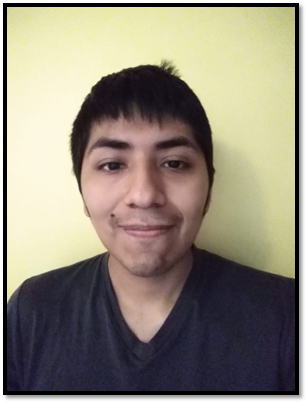
\includegraphics[width=1.72in,height=2.25in]{./media/image4.png}
\end{figure}


%%%%%%%%%%%%%%%%%%%% Figure/Image No: 4 Ends here %%%%%%%%%%%%%%%%%%%%

\par


\vspace{\baselineskip}\section*{ V.DESARROLLO}
\addcontentsline{toc}{section}{ V.DESARROLLO}

\vspace{\baselineskip}
\begin{justify}
{\fontsize{9pt}{10.8pt}\selectfont En nuestro mundo actual, donde la información es primordial en cada una de las etapas de almacenamiento, recuperación y visualización se nos presenta una necesita muy grande que consiste en el procesamiento de la información de una forma eficaz y eficiente.\par}
\end{justify}\par

\begin{justify}
{\fontsize{9pt}{10.8pt}\selectfont Una base de datos no relacional es una alternativa a que se nos presenta actualmente para este procesamiento de la información donde consiste en guardar la información en un almacenamiento de datos mucho más rápido, sin ningún tipo de estándar convencional y sobre todo escalable.\par}
\end{justify}\par


\vspace{\baselineskip}


%%%%%%%%%%%%%%%%%%%% Figure/Image No: 5 starts here %%%%%%%%%%%%%%%%%%%%

\begin{figure}[H]
	\begin{Center}
		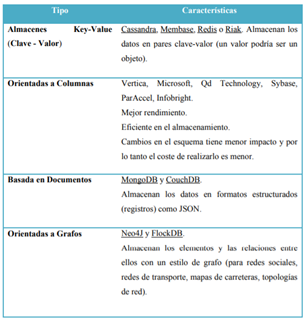
\includegraphics[width=2.81in,height=2.19in]{./media/image5.png}
	\end{Center}
\end{figure}


%%%%%%%%%%%%%%%%%%%% Figure/Image No: 5 Ends here %%%%%%%%%%%%%%%%%%%%

\par


\vspace{\baselineskip}

\vspace{\baselineskip}
\section*{Beneficios}
\addcontentsline{toc}{section}{Beneficios}

\vspace{\baselineskip}{\fontsize{9pt}{10.8pt}\selectfont Al enfocarnos en base de datos no relacionales una pregunta primordial seria: el porqué del cambio de que muchas empresas reconocidas en el mundo lo esta haciendo es migrar sus bases de datos tradicionales relacionales a un almacenamiento de datos en la mayoría libres, sin llegar a tener una estructura convencional.\par}\par

\begin{itemize}
	\item {\fontsize{9pt}{10.8pt}\selectfont En la velocidad en el tiempo de respuesta ya que los usuarios necesitan que sus necesidades sean resueltas en el menor tiempo posible\par}\par

	\item {\fontsize{9pt}{10.8pt}\selectfont La cantidad de información que se pueda almacenar\par}
\end{itemize}\par


\vspace{\baselineskip}
{\fontsize{9pt}{10.8pt}\selectfont \textbf{Ventajas de la base de datos no relacionales}\par}\par

\begin{itemize}
	\item {\fontsize{9pt}{10.8pt}\selectfont Hay bases de datos no relacionados de código abierto\par}
\end{itemize}\par

{\fontsize{9pt}{10.8pt}\selectfont Los productos de código abierto aportan beneficios a los desarrolladores como en precio, no se necesita de un servidor con grandes recursos, no tiene una estructura de datos definida ,los daos pueden ser diversos existiendo heterogeneidad\par}\par

\begin{itemize}
	\item {\fontsize{9pt}{10.8pt}\selectfont Es de escalamiento sencillo\par}
\end{itemize}\par

{\fontsize{9pt}{10.8pt}\selectfont Las base de datos no relacionales buscan una manera de añadir más servidores para manejar más cargas de datos, permitiendo a las empresas una distribución de los equipos dependiendo de las actividades a realizar.\par}\par

\begin{itemize}
	\item {\fontsize{9pt}{10.8pt}\selectfont Economía\par}
\end{itemize}\par

{\fontsize{9pt}{10.8pt}\selectfont Las base de datos no relacionales utilizan servidores de bajo costo para la administración de los datos y el volumen de las transacciones que realicen. El costo por gigabyte por segundo para estas bases puede ser mucho menor que el costo de los RDBMS , lo que le permite almacenar y procesar más datos a un precio mucho más bajo, pudiendo así añadir maquinas según sean las necesidades de la empresa\par}\par

\begin{itemize}
	\item {\fontsize{9pt}{10.8pt}\selectfont No generan cuellos de botella\par}
\end{itemize}\par

{\fontsize{9pt}{10.8pt}\selectfont Las base de datos relacionales tienen este problema ya que estos tienen que transcribir cada sentencia para ser ejecutadas incluyendo las sentencias complejas, además de un nivel de ejecución más preciso para llevar a cabo por lo que constituye un punto de entrada común, único, y conflictivo en base a rendimiento.\par}\par



%%%%%%%%%%%%%%%%%%%% Figure/Image No: 6 starts here %%%%%%%%%%%%%%%%%%%%

\begin{figure}[H]
	\begin{Center}
		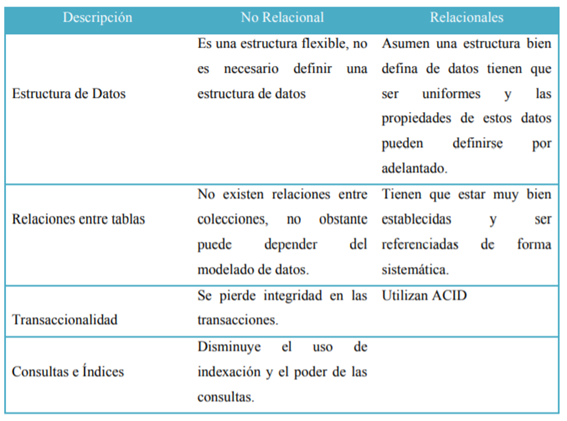
\includegraphics[width=3.19in,height=2.37in]{./media/image6.png}
	\end{Center}
\end{figure}


%%%%%%%%%%%%%%%%%%%% Figure/Image No: 6 Ends here %%%%%%%%%%%%%%%%%%%%

\par

{\fontsize{9pt}{10.8pt}\selectfont  \par}\par

{\fontsize{9pt}{10.8pt}\selectfont Se hizo el uso de base de datos no relacional en un proyecto de investigacion relacionada al estudio cientifico del espacio para esa investigacion se requerio de una base de datos no relacional\par}\par

{\fontsize{9pt}{10.8pt}\selectfont Diseño e implementación de un prototipo de una base de datos no relacional con manejo de flujo eficiente en el contexto de alertas astronómicas\par}\par

{\fontsize{9pt}{10.8pt}\selectfont Base de datos NoSql\par}\par

{\fontsize{9pt}{10.8pt}\selectfont Debido a la cantidad de datos que se generan en la actualidad, ya sea en las redes sociales, en investigaciones científicas, en los telescopios, etc., los sistemas de gestión de bases de datos relacionales o SGBD comenzaron a presentar dificultades en los aspectos de escalabilidad y rendimiento, es por esto que surgieron las bases de datos no relacionales o NoSQL (Non Structured Query Language). Estas difieren del modelo clásico de base de datos relacionales, ya que poseen una forma de almacenamiento no estructurada, son flexibles y generalmente no poseen atomicidad ni operaciones JOIN. Además, normalmente las bases de datos noSQL son sistemas distribuidos, por ende, se debe mencionar el teorema CAP (Consistency, Availability and Partition Tolerance), que, en resumen, enuncia que un sistema distribuido sólo puede garantizar 2 de las siguientes 3 características:\par}\par

{\fontsize{9pt}{10.8pt}\selectfont Consistencia: Cuando se realice una consulta, el sistema retorne la escritura más reciente de un registro dado. \par}\par

{\fontsize{9pt}{10.8pt}\selectfont ● Disponibilidad: Cuando se realice una consulta, el sistema debe retornar una respuesta en un tiempo razonable, es decir, que no retorne error ni timeout. \par}\par

{\fontsize{9pt}{10.8pt}\selectfont ● Tolerancia de particiones o tolerancia a fallos: El sistema puede seguir funcionando, aunque fallen nodos o instancias del sistema, se produzcan problemas en la comunicación entre los nodos, etc\par}\par

{\fontsize{9pt}{10.8pt}\selectfont es diseñar e implementar una base de datos no relacional, para posteriormente, realizar una simulación del streaming de las alertas astronómicas y un análisis experimental de la eficiencia de la base de datos en tiempo real.\par}\par



%%%%%%%%%%%%%%%%%%%% Figure/Image No: 7 starts here %%%%%%%%%%%%%%%%%%%%

\begin{figure}[H]
	\begin{FlushRight}		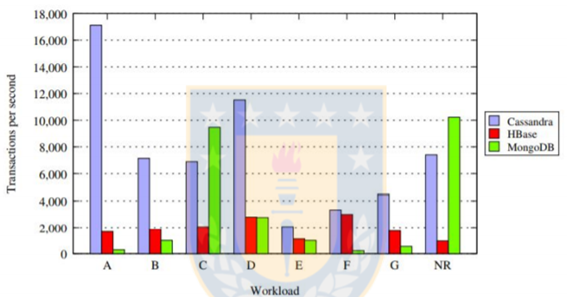
\includegraphics[width=2.96in,height=2.19in]{./media/image7.png}
	\end{FlushRight}\end{figure}


%%%%%%%%%%%%%%%%%%%% Figure/Image No: 7 Ends here %%%%%%%%%%%%%%%%%%%%

{\fontsize{9pt}{10.8pt}\selectfont realizó una evaluación de bases de datos NoSQL, en específico Cassandra, HBase y MongoDB, para aplicaciones científicas, utilizando datos tanto de bioinformática como de astronomía.\par}\par

{\fontsize{9pt}{10.8pt}\selectfont NoSQL: futuro de almacenamiento de datos\par}\par


\vspace{\baselineskip}
{\fontsize{9pt}{10.8pt}\selectfont \textbf{Tendencia actual de las NoSQL DBMS $ \vert $  Google Trends}\par}\par

{\fontsize{9pt}{10.8pt}\selectfont En el 2011, se estimó que los proveedores de la tecnología, entre todos ellos, generaron ingresos de US$\$$  20 millones, donde, aproximadamente, la mitad de estos fue logrado por 10gen (nombre del proveedor del producto MongoDB, ahora nombrado MongoDB Inc.33), pronosticando, además, que el mercado crecerá a una tasa compuesta anual del 82$\%$  hasta alcanzar los US$\$$  215 millones . Con la anterior afirmación, no solo podemos apreciar que las NoSQL en un futuro tendrán un alto crecimiento a nivel de ingresos y posicionamiento, sino, también, que MongoDB Inc con su producto MongoDB han logrado asentarse una gran base de clientes a través de su enfoque en la facilidad de adopción para el desarrollador, y volviendo su atención al tipo de necesidades actuales requeridas por las empresas.\par}\par


\vspace{\baselineskip}


%%%%%%%%%%%%%%%%%%%% Figure/Image No: 8 starts here %%%%%%%%%%%%%%%%%%%%

\begin{figure}[H]
	\begin{Center}
		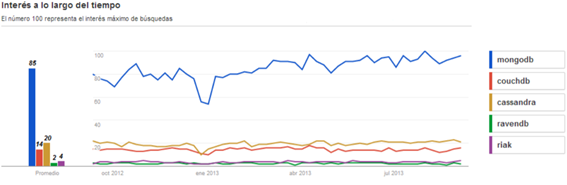
\includegraphics[width=2.81in,height=0.91in]{./media/image8.png}
	\end{Center}
\end{figure}


%%%%%%%%%%%%%%%%%%%% Figure/Image No: 8 Ends here %%%%%%%%%%%%%%%%%%%%

\par


\vspace{\baselineskip}
{\fontsize{9pt}{10.8pt}\selectfont \textbf{Tendencia actual de las NoSQL DBMS $ \vert $  Indeed}\par}\par


\vspace{\baselineskip}
{\fontsize{9pt}{10.8pt}\selectfont En este punto realizamos un análisis a las tendencias de empleo NoSQL en setiembre de 2013. La lista incluye a CassandraDB, Redis, RavenDB, SimpleDB, CouchDB, MongoDB, HBase y Riak\par}\par

{\fontsize{9pt}{10.8pt}\selectfont Como se puede evaluar, la demanda de MongoDB continúa superando a los otros productos de base de datos NoSQL, y aumentando su ventaja en los últimos meses. Cassandra continúa con un crecimiento sólido pero no puede superar a MongoDB.Está tendencia refleja no solo el crecimiento de determinados productos, sino el hecho de que las NoSQL están logrando implementarse en los negocios e impactar, agigantadamente, en las necesidades actuales de estos, puesto que requieren de los servicios de mucho más personal a lo largo del 2010.\par}\par



%%%%%%%%%%%%%%%%%%%% Figure/Image No: 9 starts here %%%%%%%%%%%%%%%%%%%%

\begin{figure}[H]
	\begin{Center}
		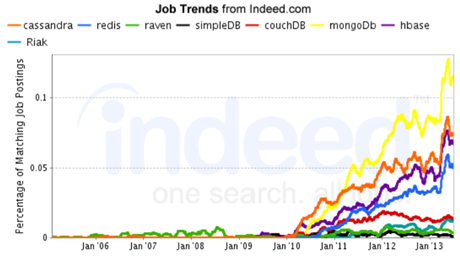
\includegraphics[width=2.81in,height=1.57in]{./media/image9.png}
	\end{Center}
\end{figure}


%%%%%%%%%%%%%%%%%%%% Figure/Image No: 9 Ends here %%%%%%%%%%%%%%%%%%%%

{\fontsize{10pt}{12.0pt}\selectfont \par}\par


\vspace{\baselineskip}

\vspace{\baselineskip}

\vspace{\baselineskip}

\vspace{\baselineskip}

\vspace{\baselineskip}
{\fontsize{9pt}{10.8pt}\selectfont \textbf{Tendencia actual de las NoSQL DBMS $ \vert $  DB-ENGINES}\par}\par

{\fontsize{9pt}{10.8pt}\selectfont MongoDB, como se puede evaluar, claramente, es el líder, y por mucho, frente a los demás productos . P\par}\par



%%%%%%%%%%%%%%%%%%%% Figure/Image No: 10 starts here %%%%%%%%%%%%%%%%%%%%

\begin{figure}[H]
	\begin{Center}
		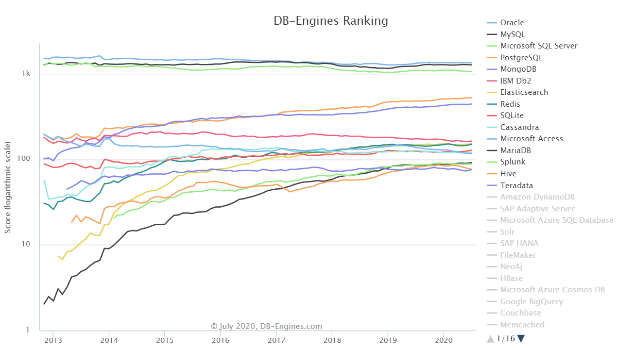
\includegraphics[width=2.81in,height=1.58in]{./media/image10.png}
	\end{Center}
\end{figure}


%%%%%%%%%%%%%%%%%%%% Figure/Image No: 10 Ends here %%%%%%%%%%%%%%%%%%%%

\par


\vspace{\baselineskip}
\begin{itemize}
	\item {\fontsize{9pt}{10.8pt}\selectfont \textbf{MongoDB: }\par}
\end{itemize}\par

{\fontsize{9pt}{10.8pt}\selectfont Estamos ante el sistema gestor de bases de datos no relacionales más \textbf{popular }y utilizado actualmente.\par}\par

{\fontsize{9pt}{10.8pt}\selectfont MongoDB es un SGBD NoSQL orientado a ficheros que almacena la información en estructuras BSON con un esquema dinámico que permite su facilidad de integración.\par}\par

{\fontsize{9pt}{10.8pt}\selectfont Empresas como Google, Facebook, eBay, Cisco o Adobe utilizan MongoDB como sistema gestor de bases de datos.\par}\par

{\fontsize{9pt}{10.8pt}\selectfont Las \textbf{principales }características de MongoDB son:\par}\par

\begin{itemize}
	\item {\fontsize{9pt}{10.8pt}\selectfont Indexación y replicación\par}\par

	\item {\fontsize{9pt}{10.8pt}\selectfont Balanceo de carga.\par}\par

	\item {\fontsize{9pt}{10.8pt}\selectfont Almacenamiento en ficheros\par}\par

	\item {\fontsize{9pt}{10.8pt}\selectfont Consultas ad hoc\par}\par

	\item {\fontsize{9pt}{10.8pt}\selectfont Escalabilidad horizontal\par}\par

	\item {\fontsize{9pt}{10.8pt}\selectfont Open Source\par}
\end{itemize}\par

{\fontsize{9pt}{10.8pt}\selectfont Como \textbf{desventaja }principal, Mongo DB no es un SGBD adecuado para realizar transacciones complejas\par}\par


\vspace{\baselineskip}
\begin{itemize}
	\item {\fontsize{9pt}{10.8pt}\selectfont \textbf{Apache Cassandra:}\par}
\end{itemize}\par

{\fontsize{9pt}{10.8pt}\selectfont Al igual que Redis (Otro SGBD conocido) Cassandra tambien utiliza almacenamiento clave-valor. Es un SGBD NoSQL distribuido y masivamente escalable.\par}\par

{\fontsize{9pt}{10.8pt}\selectfont Empresas como Facebook, Twitter, Instagram, Spotify o Netflix utilizan Cassandra.\par}\par

{\fontsize{9pt}{10.8pt}\selectfont Dispone de un lenguaje propio para las consultas denominado CQL (Cassandra Query Languaje).\par}\par

{\fontsize{9pt}{10.8pt}\selectfont Las principales características de Cassandra son:\par}\par

\begin{itemize}
	\item {\fontsize{9pt}{10.8pt}\selectfont Multiplataforma\par}\par

	\item {\fontsize{9pt}{10.8pt}\selectfont Propio lenguaje de consultas (CQL)\par}\par

	\item {\fontsize{9pt}{10.8pt}\selectfont Escalado lineal y horizontal\par}\par

	\item {\fontsize{9pt}{10.8pt}\selectfont Es un SGBD distribuido\par}\par

	\item {\fontsize{9pt}{10.8pt}\selectfont Utiliza una arquitectura peer-to-peer.\par}
\end{itemize}\par


\vspace{\baselineskip}

\vspace{\baselineskip}
{\fontsize{9pt}{10.8pt}\selectfont Características de MongoDB y Cassandra.\par}\par


\vspace{\baselineskip}


%%%%%%%%%%%%%%%%%%%% Figure/Image No: 11 starts here %%%%%%%%%%%%%%%%%%%%

\begin{figure}[H]
	\begin{Center}
		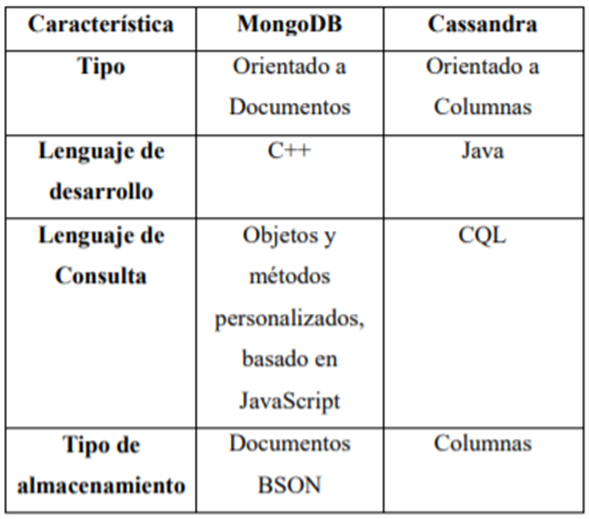
\includegraphics[width=2.82in,height=3.46in]{./media/image11.png}
	\end{Center}
\end{figure}


%%%%%%%%%%%%%%%%%%%% Figure/Image No: 11 Ends here %%%%%%%%%%%%%%%%%%%%

{\fontsize{9pt}{10.8pt}\selectfont .\par}\par



%%%%%%%%%%%%%%%%%%%% Figure/Image No: 12 starts here %%%%%%%%%%%%%%%%%%%%

\begin{figure}[H]
	\begin{Center}
		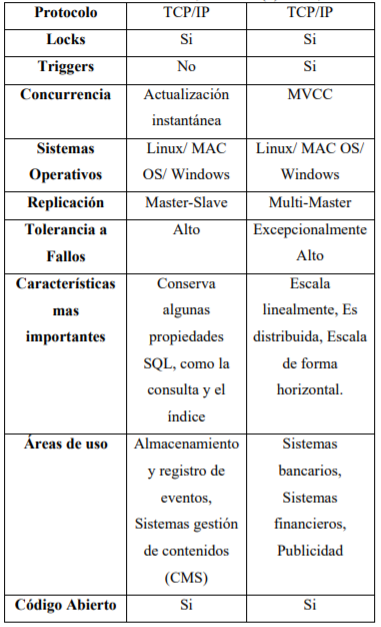
\includegraphics[width=2.81in,height=4.63in]{./media/image12.png}
	\end{Center}
\end{figure}


%%%%%%%%%%%%%%%%%%%% Figure/Image No: 12 Ends here %%%%%%%%%%%%%%%%%%%%

\par

{\fontsize{9pt}{10.8pt}\selectfont Mediante el análisis de las propiedades básicas, es posible concluir que existen similitudes cuando se trata de tipos de archivos utilizados, consultas, transacciones, locks, almacenamiento de datos, código abireto y sistemas operativos. En cuanto a términos de uso, MongoDB tiene un mejor uso para Sistemas de Gestion de Contenidos (CMS), mientras tiene consultas dinámicas con datos escritos frecuentemente. Cassandra está optimizado para almacenar e interactuar con grandes cantidades de datos que se pueden utilizar en diferentes áreas, tales como, finanzas o publicidad.\par}\par


\vspace{\baselineskip}
\textbf{\ \ \ \  VI. CONCLUCIONES}\par

\begin{itemize}
	\item {\fontsize{9pt}{10.8pt}\selectfont Existen muchos gestores de bases de datos en el mercado, pero los más usados son estos.\par}\par

	\item {\fontsize{9pt}{10.8pt}\selectfont Hay que entender bien que para elegir un SGBD más adecuado a nuestras necesidades hay que comenzar por un estudio del tipo de datos que vamos a almacenar y como lo vamos a administrar.\par}\par

	\item {\fontsize{9pt}{10.8pt}\selectfont Se determinó que al usar una base de datos no relacional en una aplicación web no transaccional al momento de realizar las consultas su tiempo de respuesta en la visualización de los resultados disminuye considerablemente por la gran cantidad de información que tiene la base\par}\par

	\item {\fontsize{9pt}{10.8pt}\selectfont El sistema de gestión de bases de datos Apache Cassandra es usado ampliamente en la actualidad, debido a sus características y su funcionamiento. Lo que significa que Cassandra puede soportar tanto la ingestión, como las consultas en una situación real, sin ningún inconveniente, y en un tiempo válido para procesos.\par}
\end{itemize}\par


\vspace{\baselineskip}
{\fontsize{9pt}{10.8pt}\selectfont  \par}\par

\section{RECOMENDACIONES}
\begin{itemize}
	\item {\fontsize{9pt}{10.8pt}\selectfont Entre los SGBD citados encontraremos alguno que se adapte a nuestras necesidades de acuerdo a la inversión a realizar, el volumen de información a almacenar, el tipo de consulta a realizar, etc.\par}
\end{itemize}\par


\vspace{\baselineskip}

\vspace{\baselineskip}
\vspace{\baselineskip}
\vspace{\baselineskip}
\vspace{\baselineskip}
\vspace{\baselineskip}\section*{VIII. BIBLIOGRAFIA}
\addcontentsline{toc}{section}{VIII. BIBLIOGRAFIA}
\href{https://revistadigital.inesem.es/informatica-y-tics/los-gestores-de-bases-de-datos-mas-usados/}{{\fontsize{9pt}{10.8pt}\selectfont https://revistadigital.inesem.es/informatica-y-tics/los-gestores-de-bases-de-datos-mas-usados/$\#$ :$ \sim $ :text=Sistemas$\%$ 20Gestores$\%$ 20de$\%$ 20bases$\%$ 20de$\%$ 20datos$\%$ 20No$\%$ 20Relacionales$\%$ 20(NoSQL),garantiza$\%$ 20completamente$\%$ 20las$\%$ 20caracter$\%$ C3$\%$ ADsticas$\%$ 20ACID}\par}\par


\vspace{\baselineskip}

\vspace{\baselineskip}
\vspace{\baselineskip}
\setlength{\parskip}{8.04pt}

\vspace{\baselineskip}

\vspace{\baselineskip}

\end{multicols}

\vspace{\baselineskip}

\vspace{\baselineskip}

\vspace{\baselineskip}

\printbibliography
\end{document}